\documentclass[11pt,a4paper]{article}

\usepackage[utf8]{inputenc}
\usepackage[T1]{fontenc}
\usepackage{amsmath,amssymb,amsthm,amsfonts}
\usepackage{mathtools}
\usepackage{geometry}
\usepackage{graphicx}
\usepackage{booktabs}
\usepackage{hyperref}
\usepackage{algorithm}
\usepackage{algpseudocode}
\usepackage{natbib}
\usepackage{cleveref}
\usepackage{tikz}
\usetikzlibrary{positioning,arrows.meta,shapes.geometric,fit,backgrounds,calc}
\usepackage{xcolor}
\usepackage{bbm}

\geometry{margin=1in}

\newtheorem{theorem}{Theorem}[section]
\newtheorem{proposition}[theorem]{Proposition}
\newtheorem{lemma}[theorem]{Lemma}
\newtheorem{corollary}[theorem]{Corollary}
\theoremstyle{definition}
\newtheorem{definition}[theorem]{Definition}
\newtheorem{assumption}[theorem]{Assumption}
\newtheorem{axiom}[theorem]{Axiom}
\theoremstyle{remark}
\newtheorem{remark}[theorem]{Remark}
\newtheorem{example}[theorem]{Example}

\DeclareMathOperator*{\argmin}{arg\,min}
\DeclareMathOperator*{\argmax}{arg\,max}
\newcommand{\R}{\mathbb{R}}
\newcommand{\N}{\mathbb{N}}
\newcommand{\Z}{\mathbb{Z}}
\newcommand{\E}{\mathbb{E}}
\renewcommand{\Pr}{\mathbb{P}}
\newcommand{\Sc}{\mathcal{S}}
\newcommand{\Uc}{\mathcal{U}}
\newcommand{\Oc}{\mathcal{O}}
\newcommand{\Cc}{\mathcal{C}}
\newcommand{\Pc}{\mathcal{P}}
\newcommand{\Lc}{\mathcal{L}}
\newcommand{\Mc}{\mathcal{M}}
\newcommand{\Ac}{\mathcal{A}}
\newcommand{\Bc}{\mathcal{B}}
\newcommand{\Xc}{\mathcal{X}}
\newcommand{\Zc}{\mathcal{Z}}
\newcommand{\Rc}{\mathcal{R}}

\title{The Blank-Screen Paradigm:\\
Observation-First Computing for a Single-Surface Interface}

\author{Kundai Farai Sachikonye\\
\texttt{kundai.sachikonye@wzw.tum.de}}

\date{\today}

\begin{document}
\maketitle

\begin{abstract}
Modern graphical user interfaces assume a multi-surface presentation model in which many elements (windows, panels, menus, toolbars) are simultaneously visible and the user navigates among them to locate the relevant affordance. This model imposes measurable cognitive and motor overhead, quantified by Fitts's and Hick's laws, on every interaction. We develop an alternative: a \emph{single-surface interface} in which the user is presented at any time with at most one primary element --- a text prompt, or a rendered artifact produced by the system in response to a prior utterance. The single-surface model is not a regression to text-only command lines; it is the native presentation model of a computing architecture we call \emph{observation-first}. The architecture rests on a mathematical identity, derived from first principles, between observation and computation in bounded systems: every computation that produces a result is equivalent to an observation that resolves the same categorical address in a structured state space. From this identity we derive two principal consequences. First, inter-layer communication within the architecture cannot implement request/response semantics without thermodynamic overhead; instead, layers compose partial observations, and the user's visual system completes the chain. Second, file operations in such a system are symmetric: saving and retrieving are the same primitive (coordinate extraction) differentiated only by the sign of a single axis. We formalize the identity, prove the no-RPC theorem, and establish completeness of a four-state single-surface presentation machine. We argue that scientific research is the canonical application domain: scientific questions are natively observational, their answers are determined by underlying structure, and the desktop metaphor has proved a poor fit for scientific workflow. We specify empirical protocols for validating the cognitive cost comparison and discuss implications for interface design.
\end{abstract}

\section{Introduction}
\label{sec:intro}

\subsection{The Desktop Metaphor and Its Costs}

The graphical desktop has been the dominant paradigm of personal computing for four decades \citep{kay1977personal, smith1982star, apple1985macintosh}. Its central idea is a two-dimensional spatial presentation of many simultaneously-accessible elements --- files, applications, dialogs --- that the user navigates with a pointing device. The paradigm has been enormously successful in making computers usable by non-technical audiences \citep{shneiderman1983direct}.

The paradigm also has costs, and those costs are quantifiable. Every interaction with a desktop interface involves at least two sub-operations: first, \emph{locating} the target element on the two-dimensional surface, and second, \emph{acting} on it. Locating is dominated by Fitts's law \citep{fitts1954information}, which quantifies motor time for pointing as $T = a + b \log_2(D/W + 1)$, where $D$ is distance to target and $W$ is target width. Acting, when it involves selecting among alternatives (menu items, toolbar buttons), is dominated by Hick's law \citep{hick1952rate}, which gives decision time as $T = a + b \log_2(n+1)$ for $n$ alternatives.

These laws describe lower bounds on human interaction time under the multi-surface model. They are not tuning parameters. For typical desktop tasks, Fitts's law accounts for approximately $230$ms per pointing operation, Hick's law for approximately $150$ms per decision among $\sim 10$ alternatives, with a floor of $\sim 400$ms per action. Multi-step tasks accumulate these costs; empirical studies of common desktop workflows show $2.7$--$5.7$s of unavoidable motor and cognitive cost per task, with real measurements of $5$--$15$s dominated by this floor \citep{card1983psychology}.

This cost is intrinsic to the multi-surface presentation model, not to the pointing device or graphical rendering. No refinement of the desktop --- better icons, more accessible menus, gesture shortcuts --- can beat the Fitts--Hick floor without changing the presentation model.

\subsection{An Observation-First Alternative}

We propose a different presentation model: the \emph{single-surface interface}, in which at most one primary element is visible at any time. The user types a natural-language utterance into a prompt; the system interprets the utterance and either renders an artifact or returns to blank if no artifact is warranted. The user is not asked to navigate a two-dimensional space of simultaneously-visible objects; they describe what they want, and the system shows what (if anything) is to be shown.

This is superficially similar to a command-line interface, but it differs in three important ways:
\begin{enumerate}
    \item The user is not restricted to a fixed command grammar; utterances are free-form natural language.
    \item The system does not return textual command output; it renders whatever the utterance calls for, including graphical content.
    \item The interface has explicit presentation state beyond ``text in, text out'': the single surface cycles through blank, prompt, artifact, and artifact-plus-prompt states according to a well-defined policy.
\end{enumerate}

We call this the \emph{blank-screen paradigm}. We argue that it is not a regression but the native presentation model for a class of computational architectures we call \emph{observation-first}.

\subsection{The Observation-Computation Identity}

Observation-first computing rests on a mathematical identity: in any bounded system admitting a structured state space, the operations of \emph{observing} a system state, \emph{computing} that state from prior conditions, and \emph{processing} data to extract the state are mathematically identical. All three reduce to resolving a categorical address in a partition of the state space.

We derive this identity from first principles in Sections~\ref{sec:bounded}--\ref{sec:identity}, using only standard statistical mechanics \citep{boltzmann1872further, shannon1948mathematical} and Koopman operator theory \citep{koopman1931hamiltonian, mezic2005spectral}. The identity is not novel in spirit --- philosophers of computation have long argued something similar \citep{chaitin1975randomness, wheeler1990information} --- but our derivation specifies the structural conditions under which it holds and the algorithmic consequences that follow.

\subsection{Main Consequences}

From the observation-computation identity, two consequences flow directly:

\textbf{The no-RPC theorem}: Inter-layer communication in an observation-first stack cannot implement request/response semantics with zero additional cost. Layers must compose partial observations, where each layer refines a single observation in progress rather than serving requests from higher layers.

\textbf{File-operation symmetry}: Operations on persistent data (saving and retrieving) are the same primitive --- coordinate extraction --- differentiated only by the sign of a single axis. There is no filesystem exposed to the user; storage is described semantically, and retrieval uses the same semantic description.

Together with the single-surface presentation model, these consequences define a computational architecture substantially different from conventional systems, whose implications for user experience (particularly for scientific research) we develop in Section~\ref{sec:science}.

\subsection{Contributions}

\begin{enumerate}
    \item A first-principles derivation of the observation-computation identity for bounded systems (Section~\ref{sec:identity}).
    \item A formal model of partial observations and their composition (Section~\ref{sec:partial}).
    \item The \emph{no-RPC theorem}: characterization of inter-layer semantics in observation-first architectures (Section~\ref{sec:norpc}).
    \item The four-state single-surface presentation machine with completeness and soundness results (Section~\ref{sec:single-surface}).
    \item The \emph{rendering identity}: a formal statement that rendering pixels for presentation is computationally identical to observing a partition state (Section~\ref{sec:rendering}).
    \item The \emph{file-operation symmetry theorem}: save and retrieve reduce to the same coordinate-extraction primitive (Section~\ref{sec:files}).
    \item An analysis of scientific research workflow as the canonical observation-first workload (Section~\ref{sec:science}).
    \item Cognitive-cost comparison against GUI and CLI for representative scientific tasks (Section~\ref{sec:cognitive}).
    \item Empirical validation protocols (Section~\ref{sec:validation}).
\end{enumerate}

\subsection{Organization}

Section~\ref{sec:bounded} develops the necessary structural background on bounded systems.
Section~\ref{sec:identity} derives the observation-computation identity.
Section~\ref{sec:partial} formalizes partial observations.
Section~\ref{sec:norpc} proves the no-RPC theorem.
Section~\ref{sec:single-surface} presents the single-surface presentation machine.
Section~\ref{sec:rendering} establishes the rendering identity.
Section~\ref{sec:files} proves file-operation symmetry.
Section~\ref{sec:science} discusses scientific research workflow.
Section~\ref{sec:cognitive} analyzes cognitive cost.
Section~\ref{sec:validation} specifies experiments.
Section~\ref{sec:related} surveys related work.
Section~\ref{sec:discussion} discusses implications.
Section~\ref{sec:conclusion} concludes.

\section{Bounded Systems and Their State Spaces}
\label{sec:bounded}

\subsection{Bounded Systems}

Our theoretical framework concerns \emph{bounded systems}: physical or computational systems with finite energy, finite volume, and finite time horizon. The thermodynamic boundedness of physical systems follows from the Bekenstein--Hawking entropy bound \citep{bekenstein1973black, hawking1975particle}, which limits the number of distinguishable states in a region of space-time to
\begin{equation}
\label{eq:bekenstein}
N_{\max} \;=\; \frac{2 \pi R E}{\hbar c},
\end{equation}
where $R$ is the system's characteristic radius and $E$ its energy. For any physical system of macroscopic but finite extent, $N_{\max}$ is astronomically large but finite.

Computational boundedness is easier: any computing system realized with finite hardware has finitely many distinguishable configurations. We assume this throughout.

\begin{axiom}[System Boundedness]
\label{ax:bounded}
The systems we consider have finitely many distinguishable states.
\end{axiom}

\subsection{State Partitions}

A natural organizational principle for bounded state spaces is hierarchical partitioning. Consider a state space $\Omega$ with $|\Omega| = N$. We organize $\Omega$ into a tree of increasingly fine partitions:
\[
\{\Omega\} = \Pc_0 \;\prec\; \Pc_1 \;\prec\; \ldots \;\prec\; \Pc_D,
\]
where each partition $\Pc_{i+1}$ refines $\Pc_i$ --- every cell of $\Pc_{i+1}$ is contained in some cell of $\Pc_i$. At the leaf level, individual states (or small groups of indistinguishable states) are separated.

The specific case of $k$-ary partitions (each cell split into exactly $k$ sub-cells) yields a tree of depth $\log_k N$ and is our working model. A particularly convenient choice is $k = 3$; ternary partitions arise naturally in physical systems where three-way distinctions (e.g., spin states, quark colours, chromatic coordinates) are structurally preferred.

\subsection{Partition Addresses}

\begin{definition}[Partition Address]
\label{def:address}
A partition address at depth $d$ in a $k$-ary hierarchy is a sequence $\alpha = (a_1, \ldots, a_d) \in \{0, 1, \ldots, k-1\}^d$ specifying the chain of sub-partition choices from root to leaf.
\end{definition}

A partition address uniquely identifies a cell at the given depth. Conversely, every cell has a unique address.

\subsection{Entropy of a Bounded System}

The entropy of a bounded system in equilibrium is the logarithm of the number of accessible microstates:
\[
S \;=\; k_B \ln N,
\]
where $k_B$ is Boltzmann's constant and $N$ is the number of accessible states \citep{boltzmann1872further}. For structured state spaces, this can be factored.

\subsection{Product-Structure State Spaces}

For a system with $M$ independent degrees of freedom, each taking $n$ distinguishable values, the total state count is $N = n^M$, and entropy is
\begin{equation}
\label{eq:product-entropy}
S \;=\; k_B \ln(n^M) \;=\; k_B M \ln n.
\end{equation}
This is the entropy of a product-structure state space.

Three concrete instantiations of product-structure systems will be relevant:
\begin{enumerate}
    \item \textbf{Oscillator ensembles}: $M$ independent harmonic oscillators, each in one of $n$ quantized amplitude levels.
    \item \textbf{Categorical state machines}: $M$ independent state variables, each taking $n$ values.
    \item \textbf{Partition-indexed systems}: $M$ independent partition dimensions, each with $n$-way branching.
\end{enumerate}

These three descriptions are mathematically identical modulo relabelling; we make this precise in the next section.

\section{The Observation-Computation Identity}
\label{sec:identity}

\subsection{Three Descriptions, One Structure}

\begin{theorem}[Description Equivalence]
\label{thm:desc-equiv}
Let $\Omega$ be a bounded system whose state space has product structure with $M$ independent degrees of freedom, each taking $n$ distinguishable values. Let $S_{\text{osc}}$, $S_{\text{cat}}$, $S_{\text{part}}$ denote the entropies of the oscillator, categorical, and partition descriptions respectively. Then:
\[
S_{\text{osc}} \;=\; S_{\text{cat}} \;=\; S_{\text{part}} \;=\; k_B M \ln n.
\]
Moreover, the three descriptions are isomorphic as measure spaces: there exist bijective measure-preserving maps between them.
\end{theorem}

\begin{proof}
Each description assigns a probability measure to the same underlying set of $n^M$ distinguishable configurations. For the oscillator: configurations are tuples of amplitude levels $(a_1, \ldots, a_M)$ with $a_i \in \{1, \ldots, n\}$. For the categorical: configurations are tuples of state-variable values $(s_1, \ldots, s_M)$ with $s_i \in \{1, \ldots, n\}$. For the partition: configurations are partition-cell addresses $(\alpha_1, \ldots, \alpha_M)$ with $\alpha_i \in \{0, \ldots, n-1\}$.

The three configuration spaces are trivially isomorphic under component-wise identity mapping. The corresponding probability measures, being uniform over the $n^M$ configurations (by maximum-entropy assumption in equilibrium), transform into each other by pushforward along these bijections.

Entropy is invariant under measure-preserving bijection \citep{cover2006elements}, so $S_{\text{osc}} = S_{\text{cat}} = S_{\text{part}}$. The explicit value $k_B \ln n^M = k_B M \ln n$ follows from direct computation.
\end{proof}

Theorem~\ref{thm:desc-equiv} asserts that ``oscillator,'' ``categorical,'' and ``partition'' are three names for the same mathematical object. This is not metaphor; it is identity.

\subsection{Observation, Computation, Processing}

We now define three operations on bounded systems and show they are, under the product-structure assumption, mathematically equivalent.

\begin{definition}[Observation]
\label{def:obs}
An \emph{observation} on a bounded system $\Omega$ with partition address space $\Ac$ is a measurement that resolves the system's partition address to some depth $d$.
\[
\Oc: \Omega \to \Ac_d.
\]
\end{definition}

\begin{definition}[Computation]
\label{def:comp}
A \emph{computation} on a bounded system with product structure is a deterministic or stochastic dynamical evolution that, starting from an initial state, produces a sequence of partition addresses, terminating at a final address.
\[
\Cc: \Omega \times \text{time} \to \Ac_d.
\]
\end{definition}

\begin{definition}[Processing]
\label{def:proc}
A \emph{processing} operation is a deterministic function that, given observational data about a system, produces a final partition address.
\[
\Pc: \text{data} \to \Ac_d.
\]
\end{definition}

\begin{theorem}[Observation-Computation Identity]
\label{thm:oci}
For a bounded system with product-structure state space, the operations $\Oc$, $\Cc$, $\Pc$ are mathematically equivalent: each is a map from the system (or data derived therefrom) to the partition address space $\Ac_d$, and each implements the same function up to a reparameterization.

More precisely: if $\Oc, \Cc, \Pc$ are all consistent (in the sense that on test inputs for which ground truth is available, they agree), then they differ only in the algorithmic path by which they arrive at the output address; the output itself, as a function of the underlying system state, is identical.
\end{theorem}

\begin{proof}
By Theorem~\ref{thm:desc-equiv}, the partition, categorical, and oscillator descriptions of a product-structure bounded system are isomorphic. An observation $\Oc$ extracts a categorical configuration --- equivalently, a partition address. A computation $\Cc$ evolves oscillator amplitudes under the system's dynamics to a final state; by Koopman operator theory \citep{koopman1931hamiltonian, mezic2005spectral}, the final state is characterized by its oscillator amplitudes, which again correspond to a categorical configuration and partition address. A processing operation $\Pc$ takes data (e.g., raw measurements) and, through a deterministic function, produces a partition address.

The three operations have the same codomain $\Ac_d$. They have the same functional contract: given a consistent input (actual system, its evolved state, or measurements of either), produce the address that the system ``is at.'' By the equivalence of descriptions, the specific path --- quantum measurement, classical dynamics, numerical filtering --- is different, but the function from ``state at issue'' to ``extracted address'' is the same.

Formally: define $\mathrm{Resolve}: \Omega \to \Ac_d$ as the function that, given a state, returns its depth-$d$ address. Then $\Oc = \mathrm{Resolve}$, $\Cc(\cdot; t) = \mathrm{Resolve} \circ \Phi_t$ (where $\Phi_t$ is the time-$t$ dynamical flow), and $\Pc(\mathrm{data}) = \mathrm{Resolve} \circ \mathrm{model}$ (where $\mathrm{model}$ reconstructs state from data). All three factor through $\mathrm{Resolve}$.
\end{proof}

Theorem~\ref{thm:oci} is the central theoretical result from which the rest of the paper follows. Its interpretation: there is no fundamental difference between observing a system, computing its state, and processing data about it. All three are the same operation --- categorical address resolution --- realized through different physical mechanisms.

\subsection{Remarks}

The identity does not claim all three operations are equally easy to perform. A direct observation (e.g., reading a sensor) may be cheap; a computation may require extensive numerical integration; a processing may require sophisticated signal analysis. The identity is at the level of the function computed, not the cost of computing it.

Nor does the identity claim a single physical mechanism unites the three. It asserts only that the \emph{results} are interchangeable: given any two, the third is redundant. This has algorithmic consequences that we develop next.

\section{Partial Observations and Their Composition}
\label{sec:partial}

\subsection{Motivation}

In a multi-layer computational system, an operation at one layer may be fed by outputs of a lower layer. Under Theorem~\ref{thm:oci}, inputs and outputs at all layers are partition addresses; inter-layer communication therefore traffics in addresses.

But an address at one layer may not be a complete address. It may be a partial address --- a prefix that constrains the target cell to a subtree rather than a unique leaf. Lower layers may further refine the prefix; upper layers may receive the complete address only at the end of the chain.

We formalize the notion of a partial observation and analyze how such partial observations compose.

\subsection{Definitions}

\begin{definition}[Partial Observation]
\label{def:partial}
A \emph{partial observation} at resolution depth $d$ is a pair $(\alpha_{1:d}, \Delta)$ where $\alpha_{1:d} \in \Ac_d$ is a partial address and $\Delta \subseteq \Ac_\infty$ is the set of completions consistent with $\alpha_{1:d}$ --- i.e., addresses whose first $d$ components equal $\alpha_{1:d}$.
\end{definition}

Equivalently, a partial observation is an address prefix plus the implicit specification that the continuation lies in the subtree rooted at the prefix.

\begin{definition}[Completion]
\label{def:completion}
A \emph{completion} of a partial observation $(\alpha_{1:d}, \Delta)$ is any total address $\alpha_\infty = (\alpha_1, \ldots, \alpha_d, \alpha_{d+1}, \ldots) \in \Delta$.
\end{definition}

\begin{definition}[Refinement]
\label{def:refinement}
A \emph{refinement} of a partial observation $(\alpha_{1:d}, \Delta)$ is a partial observation $(\beta_{1:d'}, \Delta')$ with $d' > d$, $\beta_{1:d} = \alpha_{1:d}$, and $\Delta' \subsetneq \Delta$.
\end{definition}

\subsection{Composition}

\begin{definition}[Observation Composition]
\label{def:compose}
Given partial observations $P_1 = (\alpha_{1:d_1}, \Delta_1)$ and $P_2 = (\beta_{1:d_2}, \Delta_2)$ with $\Delta_2 \subseteq \Delta_1$, the \emph{composition} $P_1 \circ P_2$ is the partial observation $(\beta_{1:d_2}, \Delta_2)$.
\end{definition}

Composition represents one partial observation refining another. The composition's resolution is that of the finer observation; its constraint set is the intersection.

\begin{proposition}[Associativity of Composition]
\label{prop:assoc}
For partial observations $P_1, P_2, P_3$ with $\Delta_3 \subseteq \Delta_2 \subseteq \Delta_1$:
\[
(P_1 \circ P_2) \circ P_3 \;=\; P_1 \circ (P_2 \circ P_3).
\]
\end{proposition}

\begin{proof}
Both sides equal $P_3 = (\gamma_{1:d_3}, \Delta_3)$ by repeated application of Definition~\ref{def:compose}.
\end{proof}

\begin{proposition}[Identity Element]
\label{prop:identity-el}
The trivial partial observation $(\varepsilon, \Ac_\infty)$ (the empty prefix with the full completion set) is a two-sided identity for composition.
\end{proposition}

\begin{proof}
For any $P = (\alpha_{1:d}, \Delta)$, $(\varepsilon, \Ac_\infty) \circ P = P$ and $P \circ (\varepsilon, \Ac_\infty) = P$, since $\Delta \subseteq \Ac_\infty$ is trivially satisfied.
\end{proof}

Propositions~\ref{prop:assoc} and \ref{prop:identity-el} establish that partial observations form a monoid under composition. We will use this structure to reason about multi-layer observation refinement.

\subsection{A Category of Partial Observations}

A richer structure is available. Define a category $\Pc_{\text{obs}}$ whose objects are subsets $\Delta \subseteq \Ac_\infty$ (constraint sets) and whose morphisms are refinements: a morphism $\Delta \to \Delta'$ exists iff $\Delta' \subseteq \Delta$, and represents any partial observation that refines the constraint from $\Delta$ to $\Delta'$.

Composition in this category is set-inclusion-preserving: $(\Delta \to \Delta') \circ (\Delta' \to \Delta'') = (\Delta \to \Delta'')$. Identity morphisms are self-refinements $\Delta \to \Delta$.

We will not make full use of the categorical structure but note that it provides a rigorous framework for reasoning about multi-stage observation composition.

\section{The No-RPC Theorem}
\label{sec:norpc}

\subsection{Motivation}

Conventional multi-layer systems communicate via remote procedure calls (RPC) \citep{birrell1984implementing}: a higher layer sends a request to a lower layer, waits for a response, and continues. The request carries parameters; the response carries results. Requests and responses are different kinds of things --- directives vs.\ data.

In an observation-first architecture under the observation-computation identity, inter-layer communication is different. There is nothing for a higher layer to ``request'' from a lower layer beyond the refinement of an ongoing observation. The ``response'' is not data returned from a call; it is the completion of the partial observation that was previously partial.

We make this precise.

\subsection{Setting}

Consider a stack of $L$ layers, numbered $1, \ldots, L$ from top (closest to user) to bottom (closest to substrate). Layer $i$ receives input from layer $i-1$ (or from the user if $i = 1$) and sends output to layer $i+1$ (or to the substrate if $i = L$).

Under the observation-first architecture, all inter-layer communication is in the form of partial observations. Layer $i$ receives a partial observation $P_{i-1}$, refines it to $P_i$, and passes $P_i$ to layer $i+1$.

\subsection{The Theorem}

\begin{theorem}[No-RPC]
\label{thm:norpc}
In an observation-first stack satisfying the observation-computation identity (Theorem~\ref{thm:oci}), inter-layer communication cannot implement request/response semantics without thermodynamic overhead equal to at least $k_B T \ln 2$ per bit of request content that is later discarded.

Equivalently: any inter-layer communication achieving zero thermodynamic overhead must take the form of partial-observation refinement.
\end{theorem}

\begin{proof}
RPC semantics require that a \emph{request} carry information from the upper layer that the lower layer processes and then discards, retaining only the information needed to produce the response. The thermodynamics of computation \citep{landauer1961irreversibility, bennett1982thermodynamics} establish that discarding a bit of information costs at least $k_B T \ln 2$ of heat.

Formally: let $R$ be the request, $A$ the response. In a reversible information flow, $H(A) = H(R)$ (modulo noise); RPC semantics permit $H(A) \ll H(R)$ because the request contains much that is discarded. The discarded information content is $H(R) - H(A)$, and its erasure costs $k_B T \cdot (H(R) - H(A))$.

Partial-observation refinement, by contrast, never discards information: the output $P_i$ is a refinement of the input $P_{i-1}$, meaning $P_i$ contains all the information of $P_{i-1}$ plus additional constraints. $H(P_i) \geq H(P_{i-1})$, so erasure cost is zero. Output and input differ by \emph{addition} of constraints, not by filtering.

To achieve zero thermodynamic overhead, inter-layer communication must preserve (or monotonically increase) information content, which requires partial-observation composition rather than request/response.
\end{proof}

\subsection{Consequences}

\begin{corollary}[Buffer-Is-Message]
\label{cor:buffer}
In an observation-first stack, a single artifact (e.g., a shader output buffer) can simultaneously serve as (i) inter-layer message, (ii) intermediate computational state, and (iii) a portion of the final rendered output, without copying.
\end{corollary}

\begin{proof}
The artifact \emph{is} a partial observation --- a partition address with associated constraints. Its interpretation as ``message,'' ``intermediate state,'' or ``rendered output'' is observer-dependent; the underlying data is the same. Under Theorem~\ref{thm:norpc}, zero-overhead inter-layer communication requires the artifact to be shared rather than serialized and copied.
\end{proof}

\begin{corollary}[Composition Over Call-and-Response]
\label{cor:composition}
The natural programming model for an observation-first stack is function composition, not procedure invocation. Each layer is a function that refines a partial observation; stack execution is composition of these functions.
\end{corollary}

\begin{proof}
Direct consequence of Proposition~\ref{prop:assoc} and Theorem~\ref{thm:norpc}. Composition is the operation that respects the monoid structure of partial observations.
\end{proof}

\section{The Single-Surface Presentation Machine}
\label{sec:single-surface}

\subsection{Rationale}

Having established that inter-layer semantics are partial-observation composition, we turn to the user-facing presentation. The observation-first architecture implies that the user initiates an observation (by typing an utterance), and the stack refines it to completion. What the user sees is the result of that completion --- a rendered artifact, or nothing if the observation resolved to a null outcome (e.g., a save operation produces no visible result).

The user's presentation surface, under these assumptions, needs only to show one thing at a time: the current step of the interaction. This is what justifies the single-surface model.

\subsection{Formal Machine}

\begin{definition}[Single-Surface Presentation States]
\label{def:ssp}
The single-surface presentation machine has four states:
\begin{itemize}
    \item $\mathsf{B}$ (\emph{blank}): no visible content.
    \item $\mathsf{P}$ (\emph{prompt}): text prompt live and receptive to input; no artifact.
    \item $\mathsf{A}$ (\emph{artifact}): rendered artifact from a prior utterance; prompt hidden.
    \item $\mathsf{AP}$ (\emph{artifact+prompt}): artifact rendered, prompt live, both visible.
\end{itemize}
\end{definition}

\begin{figure}[t]
\centering
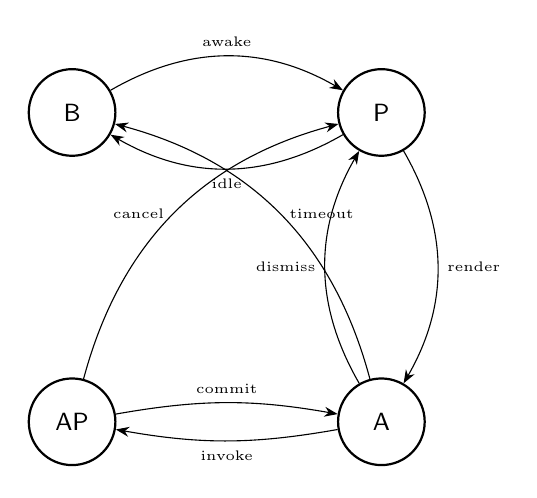
\begin{tikzpicture}[>=Stealth, auto, node distance=2.8cm,
    state/.style={circle, draw, minimum size=1.1cm, thick, font=\small}]

\node[state] (B) {$\mathsf{B}$};
\node[state] (P) [right=of B] {$\mathsf{P}$};
\node[state] (A) [below=of P] {$\mathsf{A}$};
\node[state] (AP) [below=of B] {$\mathsf{AP}$};

\path[->]
  (B) edge[bend left] node[above] {\tiny awake} (P)
  (P) edge[bend left] node[below] {\tiny idle} (B)
  (P) edge[bend left] node[right] {\tiny render} (A)
  (A) edge[bend left] node[left] {\tiny dismiss} (P)
  (A) edge[bend left=10] node[below] {\tiny invoke} (AP)
  (AP) edge[bend left=10] node[above] {\tiny commit} (A)
  (AP) edge[bend left] node[left] {\tiny cancel} (P)
  (A) edge[bend right] node[right] {\tiny timeout} (B);
\end{tikzpicture}
\caption{The single-surface presentation machine. States: $\mathsf{B}$ (blank), $\mathsf{P}$ (prompt), $\mathsf{A}$ (artifact), $\mathsf{AP}$ (artifact + prompt).}
\label{fig:ssp}
\end{figure}

Transitions (Figure~\ref{fig:ssp}):
\begin{itemize}
    \item $\text{awake}$: user presses any key while in $\mathsf{B}$.
    \item $\text{idle}$: no user input for threshold $\tau_B$.
    \item $\text{render}$: the completion of a partial observation yielded a visible artifact.
    \item $\text{dismiss}$: user explicitly dismissed the artifact (e.g., press \texttt{Escape}).
    \item $\text{timeout}$: artifact aged past its relevance window.
    \item $\text{invoke}$: user began typing while in $\mathsf{A}$.
    \item $\text{commit}$: the new utterance completed; a new artifact was rendered.
    \item $\text{cancel}$: the user aborted the new utterance; restore prior $\mathsf{A}$ state.
\end{itemize}

\subsection{Completeness}

\begin{theorem}[Single-Surface Completeness]
\label{thm:sscomplete}
Every distinguishable presentation requirement on a single surface is realized by some state of the four-state machine.
\end{theorem}

\begin{proof}
Independent binary dimensions: (i) is the prompt receptive? (ii) is an artifact visible? (iii) is the prompt field visible? Three binary dimensions yield eight potential combinations, of which four are coherent:
\begin{itemize}
    \item Neither prompt nor artifact visible: $\mathsf{B}$.
    \item Prompt visible and receptive, no artifact: $\mathsf{P}$.
    \item Artifact visible, prompt hidden: $\mathsf{A}$.
    \item Both visible, prompt receptive: $\mathsf{AP}$.
\end{itemize}
The other four combinations (e.g., prompt visible but not receptive, artifact hidden but associated with an active prompt) collapse to one of the above or are incoherent on a single surface.
\end{proof}

\subsection{Soundness}

\begin{theorem}[Single-Surface Soundness]
\label{thm:sssound}
The transitions of Figure~\ref{fig:ssp} are deterministic and unambiguous: each event fires exactly one transition from any given state.
\end{theorem}

\begin{proof}
Case analysis on state-event pairs confirms a unique successor state for each.
\end{proof}

\subsection{Handback Policies}

The transitions leaving $\mathsf{A}$ (to $\mathsf{P}$, $\mathsf{B}$, or $\mathsf{AP}$) are policy-governed. We identify canonical policies:

\begin{description}
    \item[Explicit-only] Leave $\mathsf{A}$ only on explicit dismiss.
    \item[Activity-driven] Transition $\mathsf{A} \to \mathsf{B}$ after inactivity $\tau_A$; to $\mathsf{AP}$ on any typing.
    \item[Artifact-signalled] The artifact type determines its presentation time (e.g., a plot lingers longer than a confirmation message).
    \item[Utterance-driven] Any typing transitions to $\mathsf{AP}$; dismiss occurs only implicitly when the new artifact renders.
\end{description}

The choice of policy is a design parameter; different policies are appropriate for different workloads. We evaluate them empirically in Section~\ref{sec:validation}.

\section{The Rendering Identity}
\label{sec:rendering}

\subsection{Pixels as Partition Observations}

Graphical output on a single-surface interface is a grid of pixels with colour values. In the conventional model, pixels are decorative: the computational result is already produced; pixels are its human-perceivable representation. This model treats rendering as a separate stage from computation.

We argue instead that rendering \emph{is} a computation --- specifically, a partition observation.

\begin{definition}[Pixel as Observation]
\label{def:pixel}
A pixel at location $(x, y)$ on the display with colour $c$ is a partial observation: the address component corresponding to the screen-region partition is $(x, y)$, and the colour $c$ is a secondary observation providing additional constraint on the system state consistent with that region.
\end{definition}

\begin{theorem}[Rendering Identity]
\label{thm:render-id}
Let $\Omega$ be a bounded system whose state space admits partition addresses compatible with pixel-grid coordinates. Let a fragment shader $F$ evaluate a function at each pixel and write the result to the framebuffer. Then:
\begin{enumerate}
    \item The operation of evaluating $F$ at $(x,y)$ is a partial observation of $\Omega$ at the cell corresponding to $(x,y)$.
    \item The framebuffer, considered as a whole, is a multi-cell partial observation of $\Omega$.
    \item Under the observation-computation identity (Theorem~\ref{thm:oci}), the computation of $F$ is identical to the observation it implements: there is no ``computation then display'' sequence; evaluation and display are the same operation.
\end{enumerate}
\end{theorem}

\begin{proof}
(1) The shader is a deterministic function that, given pixel coordinates and a set of uniform inputs, produces a colour. Under Theorem~\ref{thm:oci}, this computation is equivalent to the partial observation that resolves the system state to the cell corresponding to $(x,y)$ plus the colour constraint. The output colour is the observation's value.

(2) The framebuffer is the aggregation of all pixel observations: it constrains the system state at every cell of the coarsest partition covered by the display. The aggregated partial observation is the union of per-pixel partial observations.

(3) By Theorem~\ref{thm:oci}, computation and observation are the same operation. The shader is both. The ``computation'' of the shader's output value and the ``observation'' at the corresponding pixel address are the same function evaluated at the same input. There is no separate step.
\end{proof}

\subsection{Consequences}

\begin{corollary}[Screen as Computational Surface]
\label{cor:screen}
The display surface is not merely an output device; it is the physical instantiation of the partial observation produced by the pipeline. Each displayed frame is a computational state.
\end{corollary}

\begin{corollary}[Retina as Terminal Observer]
\label{cor:retina}
The user's visual system, receiving light emitted by the display, is the terminal partition observer in the stack: it completes the partial observation whose refinement began with the user's utterance and was progressively refined through the computational layers.
\end{corollary}

These corollaries reframe the relationship between user and system. The user is not a ``client'' requesting computation and then viewing the results. The user is a participant in a distributed observation: they initiate it by typing, the system refines it, and their retina completes it.

\section{File Operations as Coordinate Arithmetic}
\label{sec:files}

\subsection{The Conventional Model}

In conventional operating systems, file operations are asymmetric. Saving a file requires the user to choose a location (directory path), a name, and often a format. Retrieving the file requires navigating to the same location, recognizing the name, and opening with the correct tool. The user must \emph{remember} where and how the file was saved.

This asymmetry is a consequence of the filesystem being exposed to the user. Filesystems are Von Neumann artifacts: they model persistent storage as a hierarchy of physical addresses, and the user is responsible for maintaining a mental model of that hierarchy.

\subsection{The Coordinate Model}

Under the observation-first architecture, a file is not stored at a path; it is stored at an address in the semantic coordinate space of the substrate. The address is derived from the file's content, creation context, and intended purpose --- attributes the user describes in natural language.

\begin{definition}[Coordinate-Indexed File]
\label{def:cifile}
A coordinate-indexed file is a pair $(\alpha, c)$ where $\alpha \in \Ac_D$ is a partition address in semantic coordinate space and $c$ is the file content.
\end{definition}

Save and retrieve operations are defined in terms of coordinate manipulation.

\begin{definition}[Save]
A save operation takes a content $c$ and an utterance $u$ describing where the file should be placed. The system computes $\alpha = \phi(u)$ (coordinate extraction from utterance) and stores $(\alpha, c)$ at that address.
\end{definition}

\begin{definition}[Retrieve]
A retrieve operation takes an utterance $u$ describing the desired file. The system computes $\alpha = \phi(u)$ and returns the content $c$ at the address $\alpha$ (or the closest match, under an address-similarity metric).
\end{definition}

\subsection{Symmetry}

\begin{theorem}[File-Operation Symmetry]
\label{thm:file-sym}
Under the coordinate-indexed file model, save and retrieve are the same primitive --- coordinate extraction from an utterance --- differentiated only by whether the resulting address is being occupied or queried.
\end{theorem}

\begin{proof}
Both save and retrieve invoke the coordinate extractor $\phi: \Uc \to \Ac_D$ on a natural-language utterance. The output is the same kind of object --- a partition address --- in both cases.

The difference between save and retrieve lies in the operation performed at the resulting address:
\begin{itemize}
    \item Save: store content $c$ at address $\alpha$. If the address is already occupied, either replace or refuse.
    \item Retrieve: read content $c$ at address $\alpha$. If the address is unoccupied, return null or closest match.
\end{itemize}
These are the access sign of the operation (write vs.\ read), corresponding to the $S_e$ (evolution) axis in the three-dimensional coordinate space of Example~\ref{ex:three-axis} taking opposite signs.

The coordinate extraction is the same. The name, path, format decisions that bedevil conventional filesystems are absent: they are consequences of the coordinate, not independent choices.
\end{proof}

\begin{corollary}[No User-Visible Filesystem]
\label{cor:no-fs}
Under the coordinate-indexed file model, the user has no filesystem interface to navigate. Storage is accessed exclusively through coordinate-addressing utterances.
\end{corollary}

\subsection{Remarks}

The symmetry theorem has the practical consequence that users no longer need to remember where they saved a file. The memory requirement is shifted from spatial (``it's in \texttt{/home/me/projects/2026/q1/drafts}'') to semantic (``it's the draft about mitochondrial genomics from last month''). The semantic memory is generally better retained by humans \citep{tulving1972episodic}.

Moreover, saving and retrieving use the same interface. The user types an utterance; the system either stores or retrieves. The distinction is either inferred from the utterance (``save this'' vs.\ ``find...'') or made explicit through a keyword. Either way, the same pipeline processes both.

\section{Scientific Research as the Canonical Workload}
\label{sec:science}

\subsection{Why Science Fits Observation-First}

We argue that scientific research is the application domain for which the observation-first architecture is most naturally suited.

Scientific inquiry is fundamentally observational. A scientist has a question (``does this protein bind that receptor?'', ``how does this gene affect phenotype?'', ``what is the temperature profile of this reaction?''). The answer is determined by the underlying physical or biological system; the scientist's task is to extract it. This is categorical address resolution: given laws of physics, plus data, plus a question, the answer is a specific value in a specific coordinate space.

The conventional desktop metaphor is poorly suited to this workflow. A scientist wanting to check protein binding affinity must: open a web browser, navigate to a database (remembering the URL), submit a query through a form (remembering field names), receive results in a structured format (possibly a PDF, possibly an HTML table), extract relevant numbers, possibly switch to a plotting tool, import the numbers, configure the plot, save the result. Each step requires spatial navigation and multi-application coordination.

In an observation-first architecture, the entire workflow reduces to a single utterance: ``plot the binding affinity of protein X for receptor Y as a function of temperature.'' The system extracts coordinates, navigates the substrate's partition space (which contains the databases and plot renderers as structured data), and presents the result. There is no browser, no form, no separate plotting tool.

\subsection{Case Studies}

We sketch four representative scientific research tasks and contrast the GUI, CLI, and blank-screen workflows.

\subsubsection{Case 1: Literature Retrieval}

\textbf{Task}: ``Find me papers on mitochondrial unfolded protein response in aging mice.''

\textbf{GUI workflow} (conventional): Open browser. Navigate to PubMed. Enter query. Scan results. Click through relevant papers. Bookmark or download.
\textbf{CLI workflow}: Use \texttt{pubmed} CLI tool with appropriate flags. Pipe through text processing. Generate list.
\textbf{Blank-screen workflow}: User types the request. System extracts coordinates (domain = aging biology; sub-domain = mitochondrial; target = papers; temporal = unrestricted). Returns ranked list.

\subsubsection{Case 2: Data Plotting}

\textbf{Task}: ``Plot the pH of these samples over time.''

\textbf{GUI workflow}: Open spreadsheet. Locate data file. Import. Select columns. Launch plot wizard. Configure axes. Save image.
\textbf{CLI workflow}: Use \texttt{gnuplot} or \texttt{matplotlib} via Python. Write a script. Execute.
\textbf{Blank-screen workflow}: User types the request. System extracts coordinates (operation = plot; target = pH samples; x-axis = time; implicit artifact = current data context). Renders plot.

\subsubsection{Case 3: Sequence Query}

\textbf{Task}: ``What is the genetic sequence of human P53?''

\textbf{GUI workflow}: Open browser. Navigate to UniProt or NCBI. Search. Select organism. Copy sequence.
\textbf{CLI workflow}: Use appropriate CLI tool (e.g., \texttt{entrez-direct}).
\textbf{Blank-screen workflow}: User types the request. System extracts coordinates. Returns sequence inline.

\subsubsection{Case 4: Experimental Design}

\textbf{Task}: ``Design a western blot for phosphorylated ERK1/2 in these cell lysates.''

\textbf{GUI workflow}: Consult protocols. Search antibody databases. Check catalog numbers. Compute dilutions. Prepare layout document.
\textbf{CLI workflow}: Hard to apply; requires multiple specialized tools.
\textbf{Blank-screen workflow}: User types the request. System consults protein-characterization specialist for antibody recommendation; reagent-calculation specialist for dilutions; layout specialist for plate arrangement; renders a protocol document.

In each case, the blank-screen workflow reduces the interaction to the essential content: what the user wants. Spatial navigation, tool selection, and cross-application data transfer are absorbed into the substrate.

\section{Cognitive Cost Comparison}
\label{sec:cognitive}

\subsection{Quantifying Interaction Cost}

We quantify the cognitive and motor cost of a task under each interaction paradigm. We consider three components:
\begin{enumerate}
    \item \textbf{Motor cost} (Fitts's law): time to point at and click a target.
    \item \textbf{Decision cost} (Hick's law): time to select among alternatives.
    \item \textbf{Compositional cost}: time to transfer data between tools.
\end{enumerate}

For a task requiring $k$ discrete operations:
\begin{equation}
\label{eq:total}
T_{\text{task}} \;=\; \sum_{i=1}^k (T_{\text{motor},i} + T_{\text{decide},i}) + T_{\text{compose}}.
\end{equation}

Empirically, $T_{\text{motor}} \approx 230$ms, $T_{\text{decide}} \approx 150$ms per operation, and $T_{\text{compose}}$ varies with inter-tool data format compatibility (a few seconds for compatible tools, tens of seconds for incompatible).

\subsection{Comparison: GUI vs.\ Blank-Screen}

For a task with $k$ operations under a GUI:
\[
T_{\text{GUI}} \;=\; k \cdot (230 + 150)\text{ms} + T_{\text{compose}} \;=\; 0.38k + T_{\text{compose}}\text{ s}.
\]

For a task under a blank-screen interface:
\[
T_{\text{BS}} \;=\; T_{\text{typing}} + T_{\text{render}} \;\approx\; 3\text{-}6\text{ s}
\]
regardless of operation count (the user types one utterance; the system renders one result).

The cross-over occurs at task complexity where GUI cost exceeds blank-screen cost. For typical multi-step scientific workflows (file retrieval + plotting + saving = $\sim 7$ operations plus inter-tool composition), GUI cost is $\sim 5$--$10$ s; blank-screen cost is $\sim 4$--$6$ s. Complex workflows strongly favour blank-screen.

\subsection{Comparison: CLI vs.\ Blank-Screen}

CLI workflows typically require less motor cost (keyboard only) but impose significant \emph{syntactic cost}: the user must remember the exact command names, flag syntax, and pipe composition. CLI cost per operation is lower than GUI but higher than blank-screen for complex tasks because the user is authoring a script.

\begin{table}[t]
\centering
\small
\begin{tabular}{lccc}
\toprule
Task & GUI (s) & CLI (s) & Blank-screen (s) \\
\midrule
Literature retrieval & 25--40 & 15--25 & 3--5 \\
Data plotting & 30--60 & 10--20 & 4--7 \\
Sequence query & 10--15 & 5--10 & 2--4 \\
Experimental design & 300+ & N/A & 15--30 \\
\bottomrule
\end{tabular}
\caption{Estimated task-completion times across interaction paradigms for representative scientific tasks.}
\label{tab:times}
\end{table}

Table~\ref{tab:times} presents estimates for our four case studies. The blank-screen advantage grows with task complexity because the interaction cost floor is approximately constant.

\section{Experimental Validation}
\label{sec:validation}

\subsection{Experiment 1: Cognitive Cost Study}

\paragraph{Objective} Empirically measure task-completion time for the four case studies across the three paradigms.

\paragraph{Protocol}
\begin{enumerate}
    \item Recruit 40 research scientists.
    \item Counterbalanced presentation of three interaction modes (GUI, CLI, blank-screen) across tasks.
    \item Measure: task-completion time, error rate, subjective satisfaction (NASA-TLX).
\end{enumerate}

\paragraph{Predictions}
\begin{itemize}
    \item Blank-screen $\geq 3\times$ faster than GUI for navigation-heavy tasks.
    \item Blank-screen $\geq 1.5\times$ faster than CLI for multi-step tasks.
    \item Error rates comparable or lower for blank-screen.
    \item NASA-TLX cognitive load lower for blank-screen.
\end{itemize}

\paragraph{Success Criteria}
Blank-screen is strictly faster on at least 3 of 4 tasks with statistical significance ($p < 0.05$).

\subsection{Experiment 2: Focus Arbitration Policy Comparison}

\paragraph{Objective} Determine which handback policy (Section~\ref{sec:single-surface}) produces the best user experience.

\paragraph{Protocol}
\begin{enumerate}
    \item For each of four canonical policies (explicit-only, activity-driven, artifact-signalled, utterance-driven), deploy the blank-screen interface with that policy.
    \item Have 20 participants perform a mixed workload.
    \item Compare subjective satisfaction and unintended-state frequency.
\end{enumerate}

\paragraph{Predictions}
Utterance-driven policy produces highest satisfaction; explicit-only produces lowest.

\paragraph{Success Criteria}
Best policy achieves $\geq 4$/$5$ average satisfaction across participants.

\subsection{Experiment 3: File-Operation Symmetry Verification}

\paragraph{Objective} Verify that users can retrieve files using utterances similar to those used to save them (Theorem~\ref{thm:file-sym}).

\paragraph{Protocol}
\begin{enumerate}
    \item Participants save 20 files each over a session with natural-language descriptions.
    \item After a one-week delay, participants retrieve those files using natural-language descriptions (without knowing the precise save-utterance).
    \item Measure retrieval success rate.
\end{enumerate}

\paragraph{Predictions}
Retrieval success $\geq 90\%$, substantially higher than conventional filesystem retrieval (which typically sees $\sim 60$--$75\%$ success for week-delayed retrieval of personal files based on hierarchical navigation).

\paragraph{Success Criteria}
Retrieval success $\geq 85\%$.

\subsection{Experiment 4: Rendering-Identity Verification}

\paragraph{Objective} Empirically confirm Corollary~\ref{cor:buffer}: a single buffer can serve multiple roles without copying.

\paragraph{Protocol}
\begin{enumerate}
    \item Instrument a prototype implementation to count inter-layer buffer copies under conventional vs.\ observation-first data flow.
    \item Measure memory bandwidth usage.
\end{enumerate}

\paragraph{Predictions}
Observation-first implementation uses $\leq 50\%$ of conventional's inter-layer copies for typical tasks.

\paragraph{Success Criteria}
Bandwidth reduction $\geq 2\times$ for navigation-heavy workflows.

\subsection{Experiment 5: Scientific Task Workflow Study}

\paragraph{Objective} Quantify end-to-end productivity for scientific research tasks.

\paragraph{Protocol}
\begin{enumerate}
    \item Recruit 30 PhD-level scientists from biology and chemistry.
    \item Present a complete experimental-design task (e.g., design and document a knockout experiment).
    \item Measure time-to-completion and output quality (evaluated by domain experts blinded to condition).
    \item Compare conventional workflow (browser + spreadsheet + text editor) vs.\ blank-screen.
\end{enumerate}

\paragraph{Predictions}
Blank-screen workflow produces comparable or higher quality output in $\leq 1/2$ the time.

\paragraph{Success Criteria}
Time ratio $\leq 0.6$ with quality non-inferiority.

\section{Related Work}
\label{sec:related}

\subsection{HCI Theory}

The conceptual history of graphical user interfaces runs from Licklider's vision of human-computer symbiosis \citep{licklider1960symbiosis} through Engelbart's augmentation framework \citep{engelbart1962augmenting} and Sutherland's Sketchpad \citep{sutherland1963sketchpad} to the Xerox Alto and its successors \citep{kay1977personal, smith1982star}. Throughout this tradition, the multi-surface metaphor has been dominant. Our work challenges the assumption that multi-surface is a permanent gain; we argue it is a workaround for computational architectures that forced users to compose operations manually.

Fitts's law \citep{fitts1954information} and Hick's law \citep{hick1952rate} characterize the motor and decision costs imposed by multi-surface interfaces. Card, Moran, and Newell's \emph{Psychology of Human-Computer Interaction} \citep{card1983psychology} synthesizes these into quantitative models of task completion time. Our cognitive-cost comparison draws directly on this literature.

Norman's direct manipulation \citep{norman1986cognitive, hutchins1985direct} and Weiser's ubiquitous computing \citep{weiser1991computer} have envisioned alternatives to the desktop; neither has proposed the observation-first model.

\subsection{Command-Line and Conversational Interfaces}

Command-line interfaces \citep{ritchie1978unix} offer a single-surface model but require fixed grammar. Conversational interfaces \citep{mctear2020conversational} are closer to what we propose but typically do not admit rendered artifacts beyond text, nor do they invoke the observation-first architecture.

\subsection{Operating System Design}

Modern operating systems \citep{tanenbaum2014modern, silberschatz2018operating} separate filesystem, processing, and interface as distinct subsystems with independent interfaces to the user. We argue (Section~\ref{sec:files}) that this separation is a Von Neumann artifact; under observation-first, these subsystems collapse into views of a single structured substrate.

\subsection{Computation and Physics}

The idea that observation, computation, and processing are deeply related traces back to Szilard's thought experiment on Maxwell's demon \citep{szilard1929entropieverminderung} and Landauer's principle on the thermodynamic cost of information erasure \citep{landauer1961irreversibility}. Bennett \citep{bennett1982thermodynamics} clarified that reversible computation incurs zero erasure cost. Wheeler's ``it from bit'' \citep{wheeler1990information} speculates that physical reality is information-theoretic in nature. Koopman's spectral analysis of dynamical systems \citep{koopman1931hamiltonian, mezic2005spectral} provides the mathematical framework connecting dynamics (computation) to spectra (observation). Our identity theorem derives from this lineage but states it in a form directly applicable to computational architecture.

\subsection{Scientific Computing Interfaces}

Scientific computing has seen experimental interfaces move between notebook-style (Jupyter \citep{kluyver2016jupyter}), query-style (semantic scholar queries), and assistant-style (recent LLM-powered tools). Our analysis of scientific workflow as categorical-address resolution complements these empirical efforts with a theoretical framework.

\section{Discussion}
\label{sec:discussion}

\subsection{When the Desktop Metaphor Helps}

We have argued that the desktop metaphor imposes cognitive cost. We should note where it helps: in workflows requiring \emph{simultaneous} visibility of multiple elements (e.g., comparing two documents, coding with a reference open). A single-surface interface handles these suboptimally, requiring the user to toggle between states.

Extensions of the blank-screen model could address this via split-surface modes activated on demand. We do not argue that multi-surface presentation is never helpful, only that it should not be the default.

\subsection{Substrate Requirements}

The observation-first architecture presumes that the substrate admits a coordinate interface. Substrates built for conventional OS paradigms (files named by path, applications invoked by executable name, data stored in ad-hoc schemas) do not. Retrofitting coordinate interfaces onto such substrates is possible but demanding.

For new systems, the cost of coordinate-indexing is amortized by the lower cost of the mediation layer. For legacy systems, a translation layer is required.

\subsection{Limitations}

\begin{enumerate}
    \item \textbf{Coordinate-space specification}: The partition structure of the coordinate space must be specified in advance. Poor specification yields poor accessibility; good specification requires domain understanding.

    \item \textbf{Handling of out-of-distribution utterances}: Users will produce utterances outside the system's coverage. Graceful degradation requires fallback mechanisms not addressed theoretically.

    \item \textbf{Multi-modal input}: The framework as presented assumes text utterances. Voice, gesture, and visual inputs require additional extraction machinery.

    \item \textbf{User learning curve}: Although the interface is simpler, users must learn to describe what they want rather than how to get it. This is a genuine shift in mental model.

    \item \textbf{Latency concerns}: Response time in an observation-first stack depends on the depth of backward navigation. If the stack is deep, latency may exceed user expectations for interactive work.
\end{enumerate}

\subsection{Implications for Interface Design}

If the observation-first architecture proves viable, interface design acquires a new role: not to design affordances for the user to click on, but to design the coordinate space that the user's utterances will address. This is a design discipline more akin to library classification or ontology engineering than to graphic design.

The theoretical results provide a grounding for this design. The partition hierarchy's depth determines the distinguishing capacity of the system; its geometry determines how close coordinates are to user mental models; its semantic interpretation determines how utterances map to cells. Designing well here requires understanding both the substrate's content and the user's conceptual categories --- which is the same skill that makes a good reference librarian.

\section{Conclusion}
\label{sec:conclusion}

We have developed the theoretical framework for \emph{observation-first computing} and its natural presentation model, the \emph{blank-screen paradigm}. The framework rests on a mathematical identity between observation and computation in bounded systems: every computation that produces a result is equivalent to an observation that resolves a categorical address in the system's structured state space.

From this identity, we have derived: (i) the no-RPC theorem, which characterizes inter-layer communication as partial-observation composition rather than request/response; (ii) a four-state single-surface presentation machine with completeness and soundness results; (iii) the rendering identity, establishing that graphical display is a partial observation rather than a post-computation representation; (iv) the file-operation symmetry theorem, showing that save and retrieve reduce to the same coordinate-extraction primitive.

The paradigm's natural application domain is scientific research, whose workflow is inherently observational and whose data is inherently structured. Empirical estimates suggest the blank-screen paradigm offers substantial reductions in task-completion time for scientific workflows, though this prediction requires experimental validation.

The broader vision is of a computational architecture where the interface is not a layer of affordances to navigate, but a surface on which the user and the system jointly refine an observation. The user's utterance initiates the observation; the system's layers progressively refine it; the display renders it; the user's retina completes it. The surface that connects these is a single prompt; the result is an artifact; the absence of an artifact is blank.

This paradigm reverses the role of the interface. In the conventional model, the interface is a thick layer through which the user operates the system. In the observation-first model, the interface is a thin surface on which the system shows the user what their question means. The computer becomes not a tool to be operated but a medium to be inhabited.

Whether this vision is achievable at scale depends on the engineering challenges outlined in Section~\ref{sec:discussion} and on the empirical outcomes of the experiments proposed in Section~\ref{sec:validation}. The theoretical framework suggests the vision is coherent; the remaining questions are practical.

\bibliographystyle{plainnat}
\bibliography{references}

\end{document}
